\chapter{Aplicaciones del código de simulación}
\label{aplicaciones}

\section{Aplicación para el análisis paramétrico}
\label{analisis-parametrico}

Una vez que hemos confirmado que nuestro código es una herramienta válida para la simulación de un campo solar real nos proponemos a continuación aprovecharlo para realizar algunos análisis del comportamiento de los componentes del campo solar bajo diferentes condiciones o con diferetentes configuraciones. Este tipo de análisis es de especial utilidad durante la fase de diseño, cuando deben seleccionarse los diferentes componentes con el fin de alcanzar unos objetivos de rendimiento o potencia generada.

\subsection{Rendimiento del HCE en función de la radiación normal directa, $DNI$}

En la tabla \ref{tab:rendimiento_hce_dni} se resumen las principales características de algunos de los modelos de HCE más instalados hasta nuestros días. Los datos de $\varepsilon_{ext}$ son los ofrecidos por \cite{barberofresnoDesarrolloModeloTeorico2018}.

% Please add the following required packages to your document preamble:
% \usepackage{graphicx}
\begin{table}[!h]
\centering
\caption{Rendimiento en función de la radiación normal incidente para  distintos modelos de HCE}
\label{tab:rendimiento_hce_dni}
\resizebox{\textwidth}{!}{%
\begin{tabular}{cccccccc}
\parbox{5em}{\centering $DNI (W/m^2)$} &
\parbox{5em}{\centering Schott  \\ PTR70} &
\parbox{5em}{\centering Schott  \\ PTR70 2008} &
\parbox{5em}{\centering Solel \\ UVAC 2} &
\parbox{5em}{\centering  Solel \\ UVAC 3} &
\parbox{5em}{\centering  SkyFuel \\ SkyTrough DSP} &
\parbox{5em}{\centering ASE\\ HEMS08} &
\parbox{5em}{\centering NREL\\ \#6} \\ \hline
100 & 0,521 & 0,728 & 0,521 & 0,638 & 0,837 & 0,818 & 0,834 \\
200 & 0,757 & 0,862 & 0,757 & 0,816 & 0,917 & 0,907 & 0,916 \\
300 & 0,837 & 0,907 & 0,837 & 0,876 & 0,944 & 0,938 & 0,943 \\
400 & 0,876 & 0,930 & 0,877 & 0,907 & 0,958 & 0,953 & 0,957 \\
500 & 0,900 & 0,944 & 0,900 & 0,925 & 0,966 & 0,962 & 0,965 \\
600 & 0,917 & 0,953 & 0,917 & 0,937 & 0,971 & 0,968 & 0,971 \\
700 & 0,928 & 0,959 & 0,928 & 0,945 & 0,975 & 0,972 & 0,975 \\
800 & 0,937 & 0,964 & 0,937 & 0,952 & 0,978 & 0,976 & 0,978 \\
900 & 0,943 & 0,968 & 0,943 & 0,957 & 0,980 & 0,978 & 0,980 \\
1000 & 0,948 & 0,971 & 0,949 & 0,961 & 0,982 & 0,980 & 0,982
\end{tabular}%
}
\end{table}

En la \ref{fig:test1a} se muestra gráficamente cómo evoluciona el rendimiento con el aumento de $DNI$.  Se aprecia como los  modelos de última generación presentan un buen comportamiento incluso con bajas radiaciones.

\begin{figure}[!h]
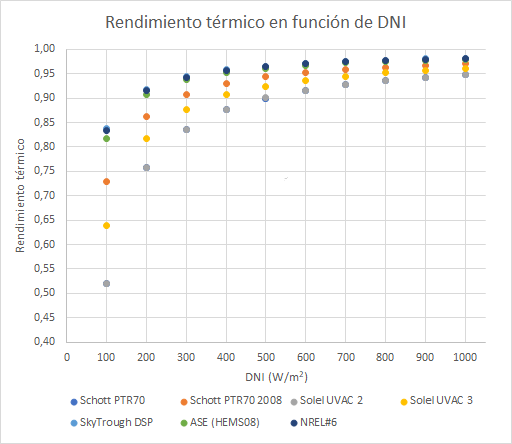
\includegraphics[width=0.9\linewidth]{images/resultados_test1a.png}
\caption{Rendimiento térmico en función de DNI para diferentes modelos de HCE} 
\label{fig:test1a}
\end{figure}

\subsection{Rendimiento del HCE en función de la temperatura de entrada}

\begin{table}[!h]
\centering
\caption{Rendimiento en función de la temperatura de entrada del HTF para diferentes modelos de HCE}
\label{tab:rendimiento_hce_tin}
\resizebox{\textwidth}{!}{%
\begin{tabular}{cccccccc}
\parbox{5em}{\centering $T_{in} (\circ C)$ } &
\parbox{5em}{\centering Schott  \\ PTR70} &
\parbox{5em}{\centering Schott  \\ PTR70 2008} &
\parbox{5em}{\centering Solel \\ UVAC 2} &
\parbox{5em}{\centering  Solel \\ UVAC 3} &
\parbox{5em}{\centering  SkyFuel \\ SkyTrough DSP} &
\parbox{5em}{\centering ASE\\ HEMS08} &
\parbox{5em}{\centering NREL\\ \#6} \\ \hline
473 & 0,975 & 0,986 & 0,974 & 0,982 & 0,993 & 0,993 & 0,993 \\
483 & 0,972 & 0,985 & 0,971 & 0,980 & 0,992 & 0,992 & 0,992 \\
493 & 0,969 & 0,983 & 0,969 & 0,978 & 0,991 & 0,990 & 0,991 \\
503 & 0,966 & 0,981 & 0,965 & 0,976 & 0,990 & 0,989 & 0,990 \\
513 & 0,963 & 0,979 & 0,962 & 0,973 & 0,988 & 0,988 & 0,988 \\
523 & 0,959 & 0,977 & 0,958 & 0,970 & 0,987 & 0,986 & 0,987 \\
533 & 0,955 & 0,975 & 0,955 & 0,967 & 0,986 & 0,984 & 0,985 \\
543 & 0,951 & 0,973 & 0,951 & 0,964 & 0,984 & 0,982 & 0,984 \\
553 & 0,946 & 0,970 & 0,946 & 0,960 & 0,982 & 0,980 & 0,982 \\
563 & 0,942 & 0,967 & 0,942 & 0,956 & 0,980 & 0,978 & 0,980 \\
573 & 0,937 & 0,964 & 0,937 & 0,952 & 0,978 & 0,976 & 0,978 \\
583 & 0,931 & 0,961 & 0,931 & 0,947 & 0,976 & 0,973 & 0,975 \\
593 & 0,925 & 0,957 & 0,926 & 0,943 & 0,974 & 0,970 & 0,973 \\
603 & 0,919 & 0,953 & 0,920 & 0,938 & 0,971 & 0,967 & 0,970 \\
613 & 0,912 & 0,949 & 0,914 & 0,932 & 0,968 & 0,963 & 0,967 \\
623 & 0,905 & 0,945 & 0,907 & 0,926 & 0,965 & 0,960 & 0,964 \\
633 & 0,898 & 0,941 & 0,900 & 0,920 & 0,962 & 0,956 & 0,961 \\
643 & 0,890 & 0,936 & 0,892 & 0,913 & 0,958 & 0,951 & 0,957 \\
653 & 0,881 & 0,931 & 0,884 & 0,906 & 0,955 & 0,947 & 0,954 \\
663 & 0,872 & 0,925 & 0,876 & 0,898 & 0,951 & 0,942 & 0,949 \\
673 & 0,863 & 0,919 & 0,867 & 0,890 & 0,946 & 0,937 & 0,945 \\
683 & 0,853 & 0,913 & 0,858 & 0,882 & 0,942 & 0,931 & 0,941
\end{tabular}%
}
\end{table}

\begin{figure}[!h]
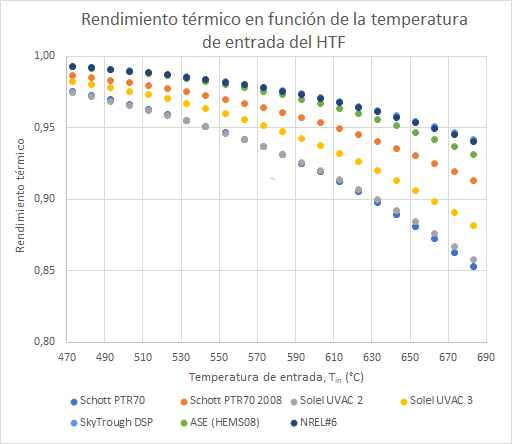
\includegraphics[width=0.9\linewidth]{images/resultados_test2a.png}
\caption{Rendimiento térmico en función de la temperatura de entrada del HTF para diferentes modelos de HCE} 
\label{fig:test2a}
\end{figure}



\subsection{Simulación con los diferentes modelos}

Comparamos ahora el resultado de simular con los tres modelos: modelo de 4º Orden, modelo de $1^{er}$ Orden y modelo simplificado. En las figuras puede verse el restultado para un día del año (se ha tomado el día 2 de marzo por tener buenas condiciones de radiación y estabilidad). 

\begin{table}[!h]
\centering
\caption{Temperaturas obtenidas en la simulación para cada modelo. Datos del día 2/3/2007. Condiciones estables y buena radiación}
\label{tab:temperaturas_modelos}
\resizebox{\textwidth}{!}{%
\begin{tabular}{ccccccc}
Hora &
\parbox{5em}{\centering DNI \\ $(W/m^2)$} &
\parbox{5em}{\centering $T_{in}$ \\ $(^\circ C)$} &
\parbox{5em}{\centering $T_{out}$  (SAM) \\ $(^\circ C)$} &
\parbox{5em}{\centering $T_{out}$ ($4^o Ord.$) \\ $(^\circ C)$} &
\parbox{5em}{\centering $T_{out}$  ($1^{er} Ord.$) \\ $(^\circ C)$} &
\parbox{5em}{\centering $T_{out}$ (Simplif.) \\  $(^\circ C)$}  \\ \hline
0:00  & 0   & 277 & 266 & 266 & 266 & 261 \\ 
1:00  & 0   & 273 & 262 & 262 & 262 & 258 \\
2:00  & 0   & 269 & 259 & 258 & 258 & 254 \\
3:00  & 0   & 265 & 255 & 255 & 255 & 251 \\
4:00  & 0   & 262 & 252 & 251 & 251 & 248 \\
5:00  & 0   & 258 & 249 & 248 & 248 & 245 \\
6:00  & 0   & 255 & 246 & 245 & 245 & 242 \\
7:00  & 234 & 252 & 263 & 243 & 243 & 240 \\
8:00  & 596 & 272 & 377 & 393 & 393 & 393 \\
9:00  & 724 & 292 & 392 & 393 & 393 & 393 \\
10:00 & 806 & 293 & 393 & 393 & 393 & 393 \\
11:00 & 859 & 293 & 393 & 393 & 393 & 393 \\
12:00 & 876 & 293 & 393 & 393 & 393 & 393 \\
13:00 & 867 & 293 & 393 & 393 & 393 & 393 \\
14:00 & 846 & 293 & 393 & 393 & 393 & 393 \\
15:00 & 781 & 293 & 393 & 393 & 393 & 393 \\
16:00 & 663 & 293 & 393 & 393 & 393 & 393 \\
17:00 & 420 & 293 & 313 & 281 & 281 & 275 \\
18:00 & 1   & 293 & 284 & 281 & 281 & 275 \\
19:00 & 0   & 298 & 282 & 285 & 285 & 280 \\
20:00 & 0   & 298 & 284 & 285 & 285 & 279 \\
21:00 & 0   & 293 & 281 & 281 & 281 & 276 \\
22:00 & 0   & 289 & 277 & 277 & 277 & 272 \\
23:00 & 0   & 284 & 273 & 273 & 273 & 268
\end{tabular}%
}
\end{table}

\begin{figure}[!h]
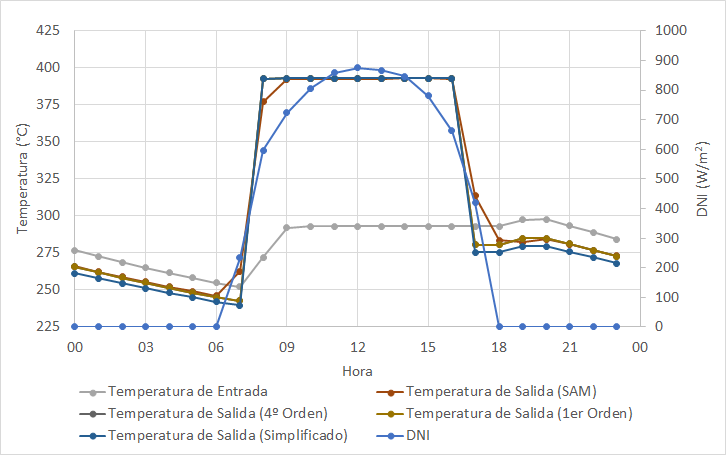
\includegraphics[width=0.9\linewidth]{images/temperaturas_modelos.png}
\caption{Temperaturas de salida obtenidas con los tres modelos} 
\label{fig:temperturas_modelos}
\end{figure}



\begin{table}[!h]
\centering
\caption{Caudales obtenidos en la simulación para cada modelo.  Datos del día 2/3/2007. Condiciones estables y buena radiación}
\label{tab:caudales_modelos}
\resizebox{\textwidth}{!}{%
\begin{tabular}{cccccc}
Hora &
\parbox{5em}{\centering DNI \\ $(W/m^2)$} &
\parbox{5em}{\centering Caudal  (SAM) \\ $(Kg/s)$} &
\parbox{5em}{\centering Caudal ($4^o Ord.$) \\ $(Kg/s)$} &
\parbox{5em}{\centering Caudal  ($1^{er} Ord.$) \\ $(Kg/s)$} &
\parbox{5em}{\centering Caudal (Simplif.) \\  $(Kg/s)$}  \\ \hline
0:00  & 0   & 204          & 204               & 204                & 204                   \\ 
1:00  & 0   & 204          & 204               & 204                & 204                   \\ 
2:00  & 0   & 204          & 204               & 204                & 204                   \\ 
3:00  & 0   & 204          & 204               & 204                & 204                   \\ 
4:00  & 0   & 204          & 204               & 204                & 204                   \\ 
5:00  & 0   & 204          & 204               & 204                & 204                   \\ 
6:00  & 0   & 204          & 204               & 204                & 204                   \\ 
7:00  & 234 & 204          & 204               & 204                & 204                   \\ 
8:00  & 596 & 530          & 514               & 516                & 518                   \\ 
9:00  & 724 & 660          & 669               & 670                & 672                   \\ 
10:00 & 806 & 648          & 661               & 663                & 664                   \\ 
11:00 & 859 & 614          & 630               & 632                & 634                   \\ 
12:00 & 876 & 599          & 617               & 619                & 621                   \\ 
13:00 & 867 & 632          & 648               & 650                & 651                   \\ 
14:00 & 846 & 699          & 714               & 716                & 718                   \\ 
15:00 & 781 & 736          & 750               & 752                & 753                   \\ 
16:00 & 663 & 599          & 620               & 622                & 624                   \\ 
17:00 & 420 & 204          & 204               & 204                & 204                   \\ 
18:00 & 1   & 204          & 204               & 204                & 204                   \\ 
19:00 & 0   & 204          & 204               & 204                & 204                   \\ 
20:00 & 0   & 204          & 204               & 204                & 204                   \\ 
21:00 & 0   & 204          & 204               & 204                & 204                   \\ 
22:00 & 0   & 204          & 204               & 204                & 204                   \\ 
23:00 & 0   & 204          & 204               & 204                & 204                   
\end{tabular}%
}
\end{table}

\begin{figure}[!h]
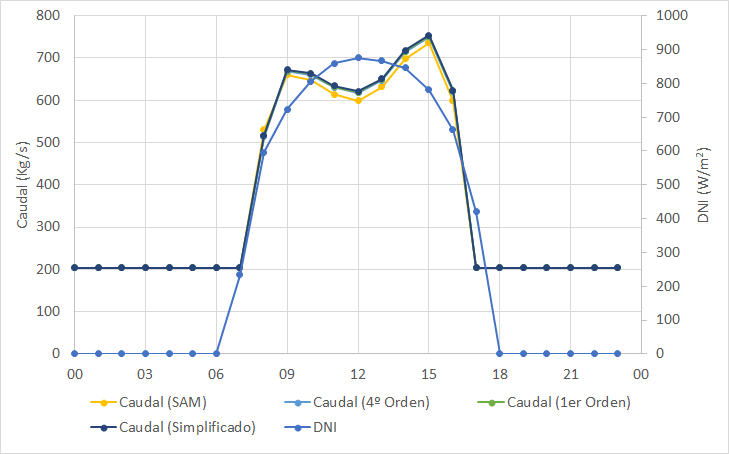
\includegraphics[width=0.9\linewidth]{images/caudales_modelos.png}
\caption{Caudales de salida obtenidos con los tres modelos} 
\label{fig:caudales_modelos}
\end{figure}


\begin{table}[!h]
\centering
\caption{Potencia térmica calculada en la simulación de cada modelo.  Datos del día 2/3/2007. Condiciones estables y buena radiación}
\label{tab:potencias_modelos}
\resizebox{\textwidth}{!}{%
\begin{tabular}{cccccc}
Hora &
\parbox{5em}{\centering DNI \\ $(W/m^2)$} &
\parbox{5em}{\centering $P_{th}$  (SAM) \\  $(MWt)$} &
\parbox{5em}{\centering $P_{th}$ ($4^o Ord.$) \\  $(MWt)$} &
\parbox{5em}{\centering $P_{th}$  ($1^{er} Ord.$) \\  $(MWt)$} &
\parbox{5em}{\centering $P_{th}$ (Simplif.) \\   $(MWt)$}  \\ \hline
0:00  & 0   & -4,9  & -5,0  & -5,0  & -6,9  \\
1:00  & 0   & -4,7  & -4,9  & -4,9  & -6,7  \\
2:00  & 0   & -4,5  & -4,8  & -4,8  & -6,5  \\
3:00  & 0   & -4,4  & -4,6  & -4,6  & -6,3  \\
4:00  & 0   & -4,2  & -4,5  & -4,5  & -6,0  \\
5:00  & 0   & -4,1  & -4,4  & -4,4  & -5,9  \\
6:00  & 0   & -3,9  & -4,3  & -4,3  & -5,7  \\
7:00  & 234 & 4,7   & -4,2  & -4,2  & -5,6  \\
8:00  & 596 & 133,1 & 149,5 & 150,1 & 150,5 \\
9:00  & 724 & 161,6 & 164,6 & 165,0 & 165,4 \\
10:00 & 806 & 157,7 & 161,2 & 161,6 & 162,1 \\
11:00 & 859 & 149,2 & 153,6 & 154,1 & 154,5 \\
12:00 & 876 & 145,5 & 150,5 & 150,9 & 151,3 \\
13:00 & 867 & 153,4 & 157,9 & 158,3 & 158,8 \\
14:00 & 846 & 170,2 & 174,2 & 174,6 & 175,0 \\
15:00 & 781 & 179,3 & 182,7 & 183,2 & 183,6 \\
16:00 & 663 & 145,6 & 151,1 & 151,6 & 152,0 \\
17:00 & 420 & 9,7   & -5,7  & -5,7  & -8,2  \\
18:00 & 1   & -4,4  & -5,7  & -5,7  & -8,1  \\
19:00 & 0   & -7,1  & -5,9  & -5,9  & -8,4  \\
20:00 & 0   & -6,3  & -5,9  & -5,9  & -8,4  \\
21:00 & 0   & -5,8  & -5,7  & -5,7  & -8,1  \\
22:00 & 0   & -5,5  & -5,5  & -5,5  & -7,8  \\
23:00 & 0   & -5,3  & -5,4  & -5,4  & -7,5 
\end{tabular}%
}
\end{table}


\begin{figure}[!h]
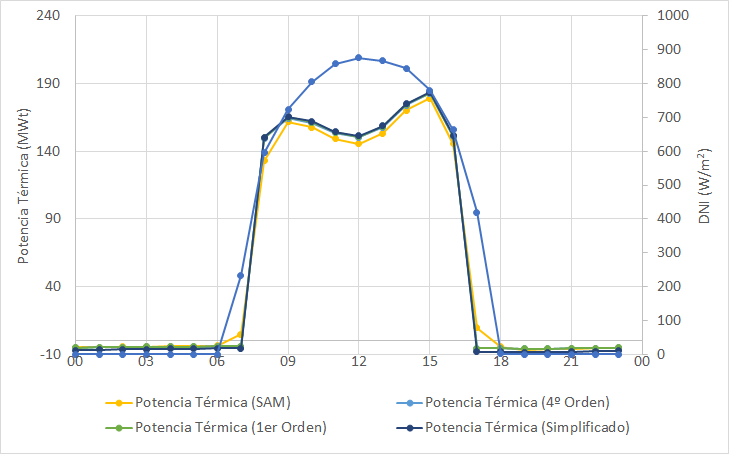
\includegraphics[width=0.9\linewidth]{images/potencias_modelos.png}
\caption{Potencia térmica obtenida con cada uno de los tres modelos} 
\label{fig:potencia_modelos}
\end{figure}


\begin{table}[!h]
\centering
\caption{Rendimientos obtenidos en la simulación de cada modelo.  Datos del día 2/3/2007. Condiciones estables y buena radiación}
\label{tab:rendimientos_modelos}
\resizebox{\textwidth}{!}{%
\begin{tabular}{ccccc}
Hora &
\parbox{5em}{\centering DNI \\ $(W/m^2)$} &
\parbox{5em}{\centering $\eta_{th}$ ($4^o Ord.$)} &
\parbox{5em}{\centering $\eta_{th}$  ($1^{er} Ord.$)} &
\parbox{5em}{\centering $\eta_{th}$ (Simplif.)} \\ \hline
0:00  & 0   & 0,000 & 0,000 & 0,000 \\
1:00  & 0   & 0,000 & 0,000 & 0,000 \\
2:00  & 0   & 0,000 & 0,000 & 0,000 \\
3:00  & 0   & 0,000 & 0,000 & 0,000 \\
4:00  & 0   & 0,000 & 0,000 & 0,000 \\
5:00  & 0   & 0,000 & 0,000 & 0,000 \\
6:00  & 0   & 0,000 & 0,000 & 0,000 \\
7:00  & 234 & 0,000 & 0,000 & 0,000 \\
 8:00  & 596 & 0,912 & 0,917 & 0,920 \\
9:00  & 724 & 0,916 & 0,920 & 0,922 \\
10:00 & 806 & 0,914 & 0,918 & 0,920 \\
11:00 & 859 & 0,910 & 0,914 & 0,917 \\
12:00 & 876 & 0,909 & 0,912 & 0,915 \\
13:00 & 867 & 0,913 & 0,916 & 0,919 \\
14:00 & 846 & 0,920 & 0,923 & 0,926 \\
15:00 & 781 & 0,923 & 0,926 & 0,928 \\
16:00 & 663 & 0,907 & 0,911 & 0,914 \\
17:00 & 420 & 0,000 & 0,000 & 0,000 \\
18:00 & 1   & 0,000 & 0,000 & 0,000 \\
19:00 & 0   & 0,000 & 0,000 & 0,000 \\
20:00 & 0   & 0,000 & 0,000 & 0,000 \\
21:00 & 0   & 0,000 & 0,000 & 0,000 \\
22:00 & 0   & 0,000 & 0,000 & 0,000 \\
23:00 & 0   & 0,000 & 0,000 & 0,000
\end{tabular}%
}
\end{table}

\begin{figure}[!h]
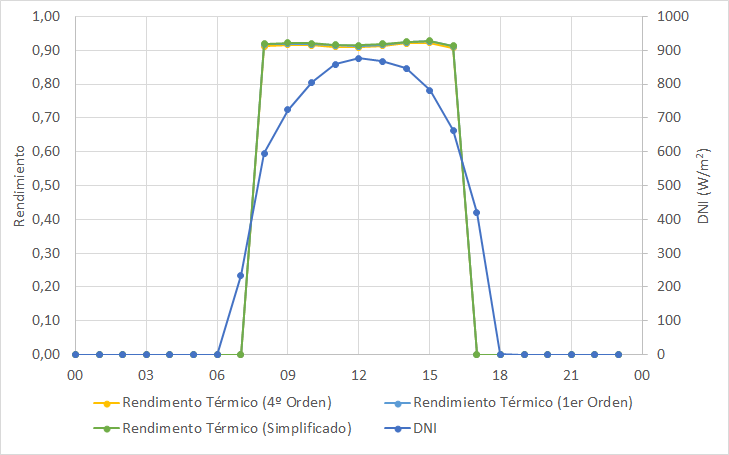
\includegraphics[width=0.9\linewidth]{images/rendimientos_modelos.png}
\caption{Rendimiento térmico para cada uno de los tres modelos} 
\label{fig:rendimientos_modelos}
\end{figure}

\subsection{Simulación cambiando el tamaño de la malla de integración}
\label{mallaintegracion}


\begin{figure}[!h]
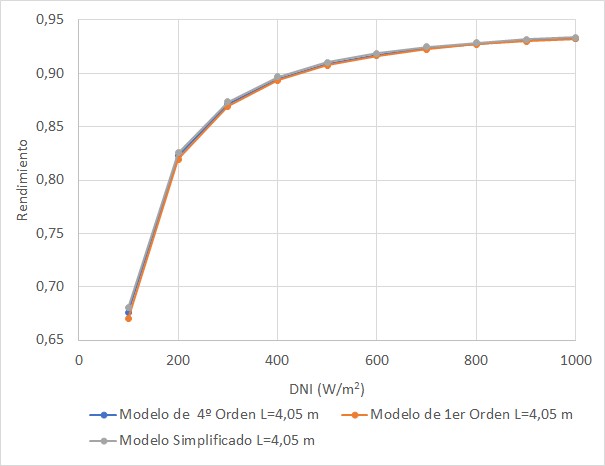
\includegraphics[width=0.9\linewidth]{images/malla0405.png}
\caption{Rendimiento calculado con cada modelo para un tamaño de malla de integración de 4,05 m} 
\label{fig:malla0405}
\end{figure}

\begin{figure}[!h]
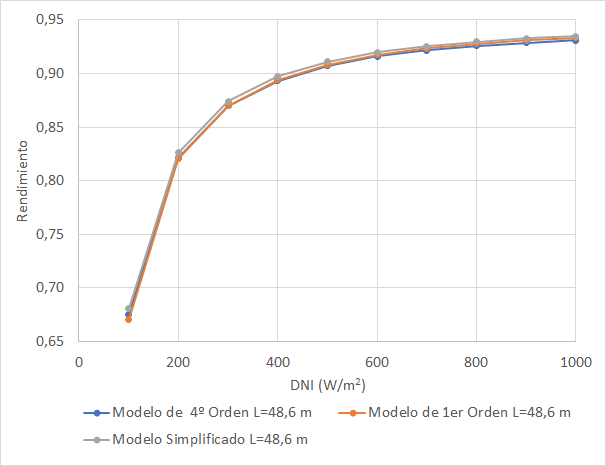
\includegraphics[width=0.9\linewidth]{images/malla4860.png}
\caption{Rendimiento calculado con cada modelo para un tamaño de malla de integración de 48,60 m} 
\label{fig:malla4860}
\end{figure}

\begin{figure}[!h]
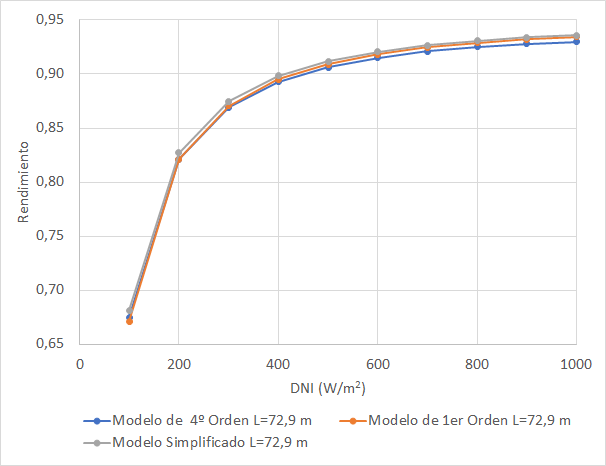
\includegraphics[width=0.9\linewidth]{images/malla7290.png}
\caption{Rendimiento calculado con cada modelo para un tamaño de malla de integración de 72,90 m} 
\label{fig:malla7290}
\end{figure}

\begin{figure}[!h]
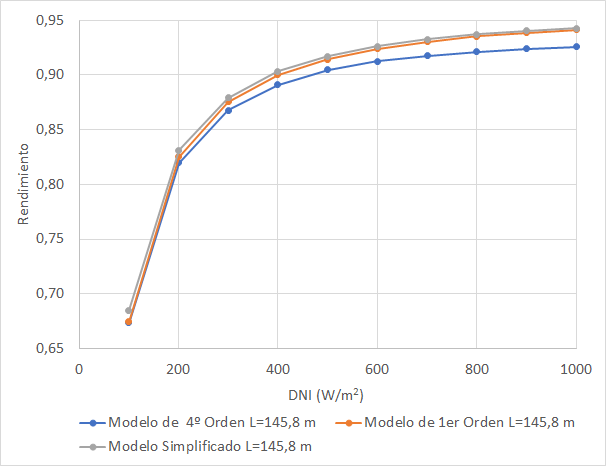
\includegraphics[width=0.9\linewidth]{images/malla14580.png}
\caption{Rendimiento calculado con cada modelo para un tamaño de malla de integración de 145,80 m} 
\label{fig:malla14580}
\end{figure}


\begin{figure}[!h]
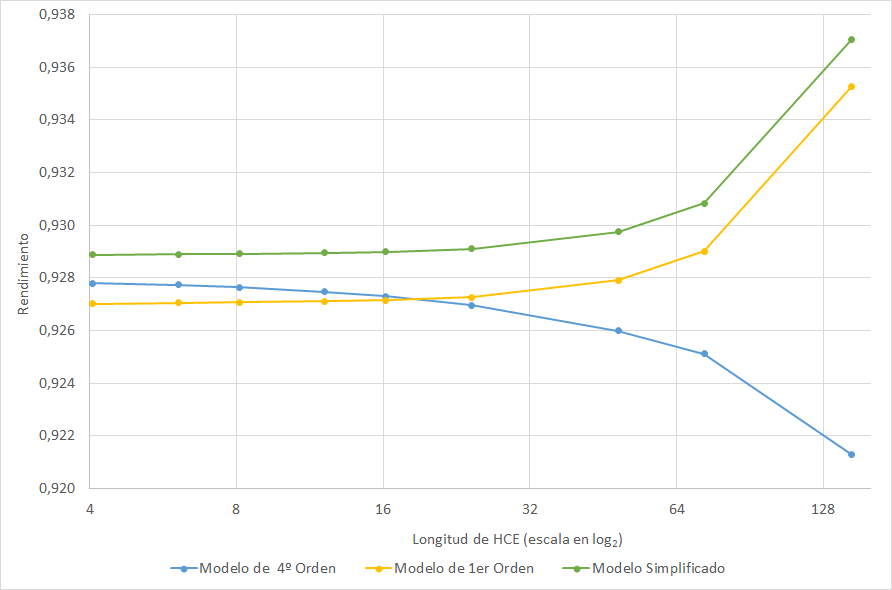
\includegraphics[width=0.9\linewidth]{images/malla_variable_DNI_800.png}
\caption{Rendimiento calculado para diferentes tamaños de malla de integración. $DNI=800 W/m^2$, $T_{in}=300 \circ C$, $\dot m = 6 kg/s$} 
\label{fig:malla_variable_DNI_800}
\end{figure}


\begin{figure}[!h]
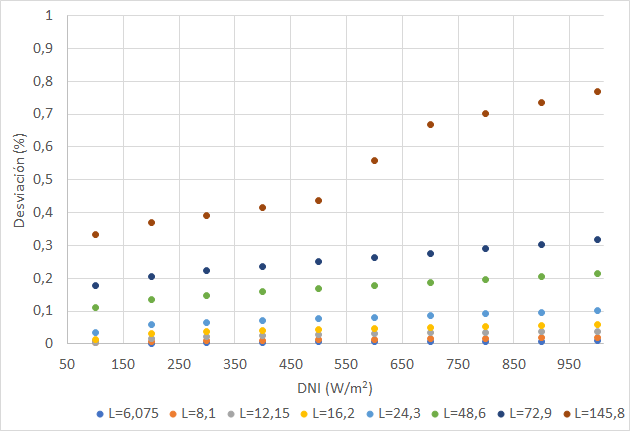
\includegraphics[width=0.9\linewidth]{images/desviacionmodel4malla.png}
\caption{Desviación, para simulaciones con el Modelo de 4º Orden, según diferentes tamaños de malla. Los valores muestran la desviación, en tanto por ciento, respecto a la simulación con una malla de 4,05 m. $T_{in}=300 \circ C$, $\dot m = 6 kg/s$} 
\label{fig:desviacionmodel4}
\end{figure}

\begin{figure}[!h]
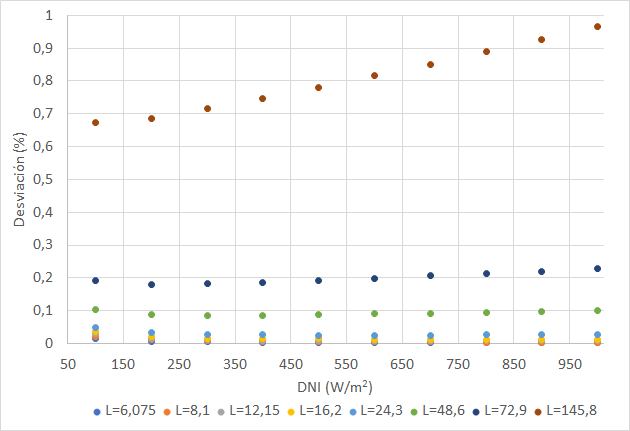
\includegraphics[width=0.9\linewidth]{images/desviacionmodel1malla.png}
\caption{Desviación, para simulaciones con el Modelo de $1^{er}$ Orden, según diferentes tamaños de malla. Los valores muestran la desviación, en tanto por ciento, respecto a la simulación con una malla de 4,05 m. $T_{in}=300 \circ C$, $\dot m = 6 kg/s$} 
\label{fig:desviacionmodel1}
\end{figure}

\begin{figure}[!h]
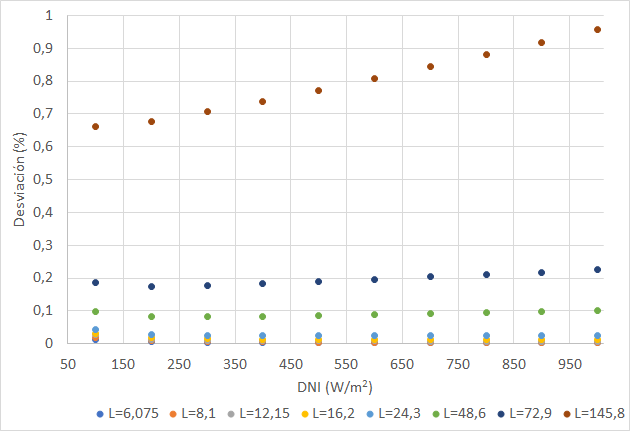
\includegraphics[width=0.9\linewidth]{images/desviacionmodelsimplificadomalla.png}
\caption{Desviación, para simulaciones con el Modelo de Simplificado, según diferentes tamaños de malla. Los valores muestran la desviación, en tanto por ciento, respecto a la simulación con una malla de 4,05 m. $T_{in}=300 \circ C$, $\dot m = 6 kg/s$} 
\label{fig:desviacionmodelsimplificado}
\end{figure}



\section{Análisis de los datos de generación de una planta solar termoeléctrica real}
\label{descripcion-central}

Finalmente emplearemos nuestro programa de simulación en un análisis del estado del campo solar de una planta termosolar real. Puesto que la simulación de sistemas externos al campo solar queda fuera de nuestro alcance, nos centraremos en los datos referentes al campo solar. En concreto, contrastaremos, para cada  hora del año, qué potencia térmica se estaba extrayendo del campo, independientemente de las causas operativas que condicionasen el funcionamiento del campo cada momento. Nuestro objetivo es comprobar si nuestra herramienta puede ser útil de cara estimar el estado global de rendimiento del campo, midiendo de alguna manera su desviación respecto a lo esperado. Realizaremos la simulación a partir de datos reales (meteorológicos y de generación) de una central termosolar, comparando el salto térmico real con el simulado. 

La configuración de campo solar que se va a utilizar a lo largo de las siguientes simulaciones está basada en las plantas termosolares Aste 1A y 1B, que se encuentran situadas en el término municipal de Alcázar de San Juan, provincia de Ciudad Real. Sus coordenadas geográficas son (39,1°N 3,16°W) y la altitud es de 651 m sobre el nivel del mar.

\begin{figure}[!h]
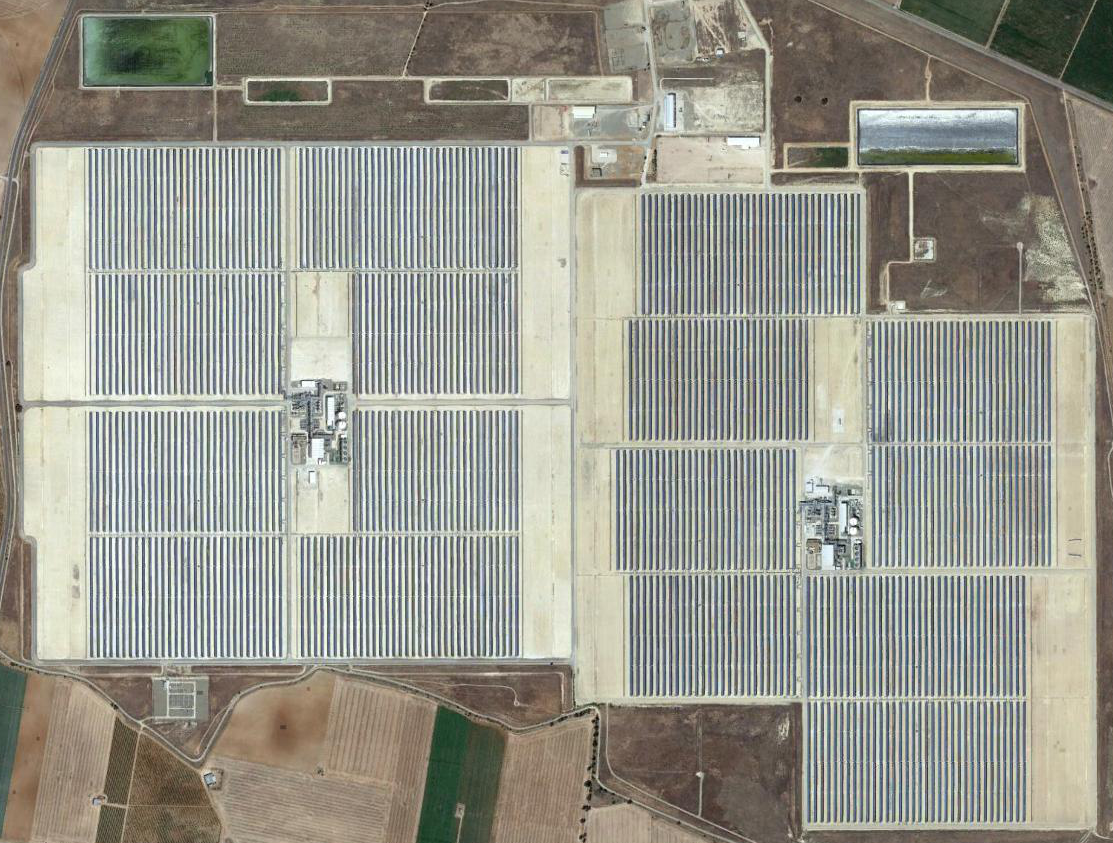
\includegraphics[width=0.9\linewidth]{images/fotoAstes.png}
\caption{Centrales Termosolares Aste 1A (izq.) y Aste 1B (der.) Fuente: Google Earth} 
\label{fig:astes}
\end{figure}

La potencia eléctrica nominal de cada una de ellas es de 49,9 MW. El proyecto inicial consideraba que las plantas contarían con almacenamiento térmico, el cual se construiría durante una segunda fase que finalmente no se llegó a ejecutar, por lo que en la actualidad solo existe generación durante las horas de sol. Se emplearán los datos de Aste 1B, cuya configuración es la siguente:

El campo solar cuenta con 120 lazos distribuidos de manera irregular en 4 subcampos. La  distancia de separación entre lazos es de 16,25 m. 

\begin{itemize}[itemsep=2pt,parsep=2pt]
\item
  Subcampo NO, 31 lazos.
\item
  Subcampo NE, 28 lazos.
\item
  Subcampo SO, 27 lazos.
\item
  Subcampo SE, 34 lazos.
\end{itemize}

Todos los lazos son idénticos, contando con 4 SCAs cada uno en una configuración tipo \(U\). El eje de seguimiento perfectamente plano se encuentra alineado en direccion N-S. Cada SCA cuenta con un total de 336 espejos de vídrio fabricados por Flabeg. 

La reflectividad de los espejos puede obtenerse a partir de los registros de mantenimiento de ese año. Llegados a este punto encontramos cierta anomalía en los valores, tal y como puede apreciarse en la \ref{fig:refelectividad}. Se observa cómo durante los meses de junio y julio el valor de la reflectividad promedio comienza a caer drásticamente hasta valores ligeramente inferiores al 60\%. Los valores van mejorando posteriormente, durante el mes de agosto, hasta alcanzar valores normales a partir de septiembre.


\begin{figure}[!h]
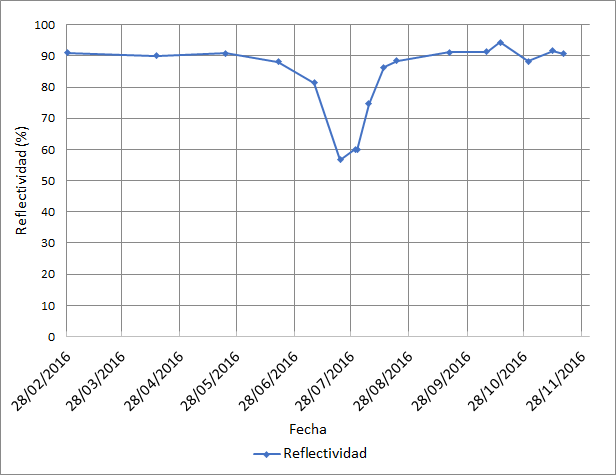
\includegraphics[width=0.9\linewidth]{images/reflectividad.png}
\caption{Reflectividad registrada durante el mantenimiento. Fuente: Propia} 
\label{fig:reflectividad}
\end{figure}

El origen de este comportamiento está en que durante ese periodo se paralizó la actividad de limpieza de espejos (por causas no aclaradas), unida a las habituales tormentas de primavera que, en esa zona, suelen venir acompañadas de viento y polvo. Una vez que se reanuda el mantenimiento y limpieza del campo solar, los valores de reflectividad vuelven a su valor habitual, alrededor del 90\%. Debe tenerse en cuenta que la limpieza de espejos de todo el campo puede requerir varias semanas para un equipo de mantenimiento compuesto por un solo camión de agua presurizada apoyado por dos operarios con un ritmo normal de limpieza de unos 8 a 10 lazos cada noche. Esta contingencia no afectó a la generación eléctrica de la planta por estar  el campo solar muy sobredimensionado.

Respecto al estado de los tubos HCE, consideraremos que se encuentran en buen estado de vacío. Los recuentos anuales efectuados en planta indican que tras 4 años de operación apenas se contabiliza una media de un HCE sin vacío por cada lazo y el número de HCE sin envolvente de vidrio es despreciable.

Los datos de las figuras \ref{fig:potencia_1b} a \ref{fig:temperatura_1b} muestran el comportamiento de la planta real para un día de buena radiación y condiciones estables. Puesto que la planta no dispone de almacenamiento energético, los efectos de las inercias de arranque y parada se aprecian claramente a primera y última hora del día, así como en los altibajos de radiación en los días inestables. En esta planta, el control de caudal lo realiza manualmente el operador de sala en base a las diferentes limitaciones que el diseño de planta impone. Especialmente importantes son los gradientes, o más propiamente dicho, las rampas de calentamiento y enfriamiento que los fabricantes de los equipos recomiendan, como es el caso de la turbina, trenes de generación, bombas principales de HTF o los propios HCEs. También existe una inercia asociada al calentamiento de tuberías y tanques de expansión y rebose.  La masa total de HTF en la planta ronda las 1300 toneladas. 

\begin{figure}[!h]
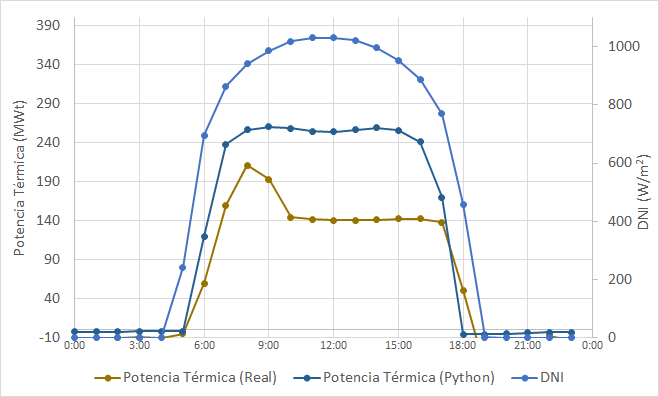
\includegraphics[width=0.9\linewidth]{images/potencia_aste1b_01052016.png}
\caption{Potencia térmica real y simulada para el día 1/5/2016. Condiciones estables y buena radiación} 
\label{fig:potencia_1b}
\end{figure}

\begin{figure}[!h]
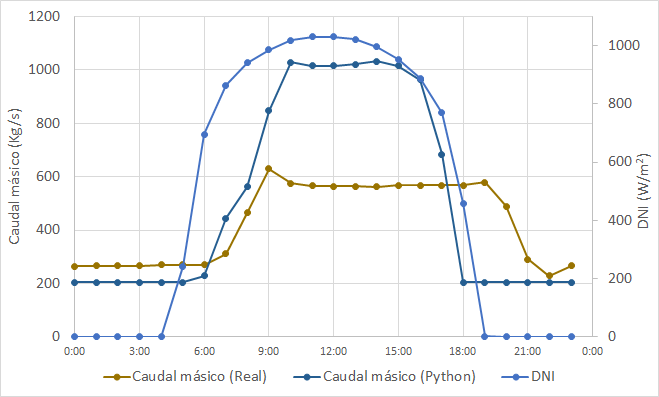
\includegraphics[width=0.9\linewidth]{images/caudal_aste1b_01052016.png}
\caption{Caudal real y simulado para el día 1/5/2016. Condiciones estables y buena radiación} 
\label{fig:caudal_1b}
\end{figure}

\begin{figure}[!h]
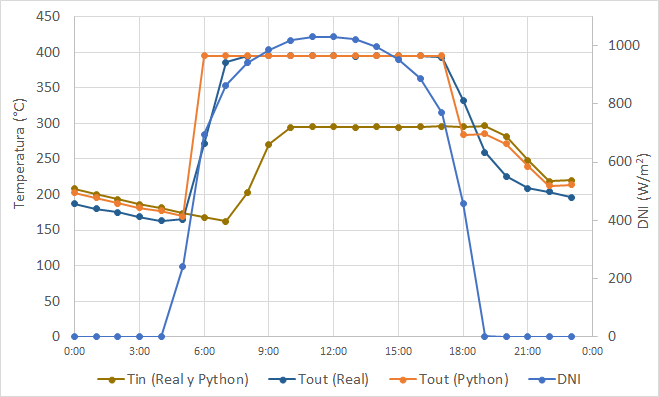
\includegraphics[width=0.9\linewidth]{images/temperatura_aste1b_01052016.png}
\caption{Temperaturas de operación reales y simulada para el día 1/5/2016. Condiciones estables y buena radiación} 
\label{fig:temperatura_1b}
\end{figure}

Para evitar que estos momentos transitorios afecten a nuestros cálculos filtraremos los datos para tener en cuenta solo aquellos momentos en los que las condiciones de generación ya son estables y todo el sistema se encuentra a plena carga. Para ellos seleccionaremos registros en los que la radiación solar directa, DNI, es superior a 700 $W/m^2$ y la temperatura de retorno al campo es muy próxima a la nominal, $T_{in}>290ºC$. Descartaremos también los datos de los meses de junio, julio y agosto debido a los valores anormales de reflectividad y los meses de noviembre a enero por incluir días en los que la planta no estaba plenamente operativa por tareas de mantenimiento y paradas programadas. Pese a todos estos descartes, queda un buen número de registros que nos permitirán analizar el rendiminento de la planta en su conjunto.

El fluido de trabajo es Dowtherm A, cuyas propiedades también se han descrito en el apartado \ref{subclases-fluid}.

Los datos meteorológicos son los recogidos a lo largo de 2016 por las tres estaciones meteorológicas con las que cuenta la planta. Al tener por triplicado las medidas de cada variable se adopta el criterio de seleccionar la mediana de las tres y no el valor medio. Esta selección la realiza el sistema de control de planta en cada momento y con este criterio se persigue conseguir una mayor robustez del sistema, pues si una estación presenta valores muy desviados de las otras dos podría darse el caso de que el valor medio estuviese muy alejado del valor  verdadero. Cuando por avería o fallo de comunicación se carece de los datos de alguna estación sí se suele adoptar el criterio de seleccionar el valor medio de las dos restantes.

\begin{figure}[!h]
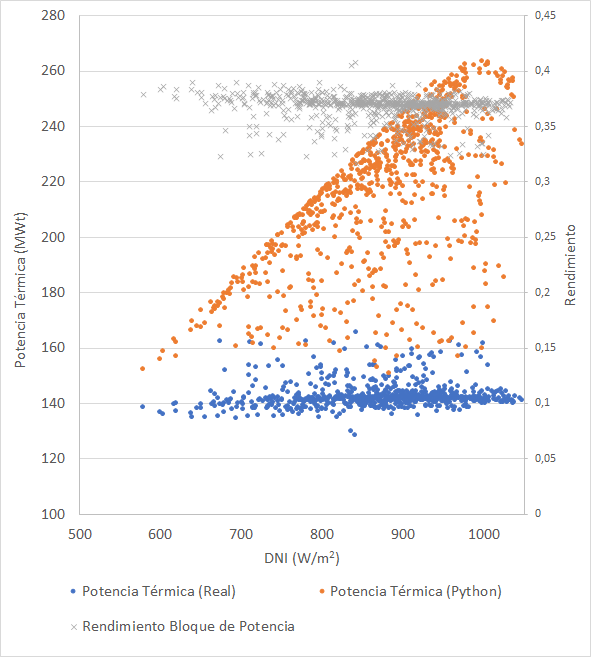
\includegraphics[width=0.9\linewidth]{images/potencia_dni_aste1b.png}
\caption{Potencia térmica real y simulada en función de DNI cuando la planta trabaja en condiciones nominales ($T_{in}$>290 ºC, $T_{out}$>390 ºC). En el eje vertical derecho se representa el rendimiento global del bloque de potencia} 
\label{fig:potenica_dni}
\end{figure}

Estado de los tubos de vacío. 

Comparar potencia térmica del campo con la disponible.
Comparar potencia benchmark para analizar pérdida de rendimiento del campo.
Pérdidas en tuberías
Potencia térmica en trenes.
Potencia turbogrupo.



 

